%% Methodology
%%=========================================

\chapter{Methodology}
\label{ch:methodology}
This chapter presents the research methodology that was used in the process of writing this thesis. Section \ref{sec:research_questions_and_approach} looks closer at the research questions which we defined in the previous chapter. Section \ref{sec:research_approaches} presents the research approach, and Section \ref{sec:research_strategy} presents our choice of research strategies. In Section \ref{sec:data_generation_methods_and_data_analysis} we present our data generation methods and how we did our data analysis.

%%=========================================

\section{Evaluating Research Questions}
\label{sec:research_questions_and_approach}
We have already presented our research goal and questions as:

\begin{description}
    \item[Research Goal]{\textit{Develop a model that is able to use signature sequences to recognize words and letters}}
    \item[Research Question 1]{\textit{Does ambiguity in character signature sequences impact recognition rates?}}
    \item[Research Question 2]{\textit{Can a signature sequence based model handle multiple fonts at the same time?}}
    \item[Research Question 3]{\textit{Can a signature sequence based model be robust to noise?}}
\end{description}

In this section we will look closer at how we give an answer to our research questions in a meaningful way:

\begin{description}
    \item[RQ1:]{It was made clear that ambiguity could be an issue early in our testing. How and why it could impact our problem is explained in Section \ref{sec:ambiguous_input}. Measuring a potential impact could be done by conducting tests and experiments to see how the recognition rates were affected by ambiguous data.}
    \item[RQ2:]{While learning to recognize words written in one font may be challenging, introducing additional fonts will almost certainly increase the difficulty, resulting in a more complex problem. Whether or not a model is capable of handling this can, similarly to \textbf{RQ1}, be answered by running tests with text written in multiple fonts and see how the recognition rates were affected. Sections \ref{sec:tuning_input_data} and \ref{sec:use_of_fonts} explains how we can tune the input and how typography techniques may affect recognition.}
    \item[RQ3:]{While clean and well-formatted data is preferable, we may not always be so lucky that our data is completely noise free. Noise-induced data is also much more ``realistic'', in a real world perspective than 100\% noise-free data. Investigating how well a model can handle certain degrees of noise is interesting, as it could say something about its robustness. Investigating this could be done by running tests and introduce noise increasingly until the recognition rates deteriorate beyond a certain point.}
\end{description}

%%=========================================

\section{Research Approaches}
\label{sec:research_approaches}
We chose to follow the research process presented by \cite{oates2005researching}. Figure \ref{fig:model_research_process} gives an overview of this process and its components. The overview illustrates how to form different research approaches by mixing and matching various types of strategies, data generation methods, and types of data analysis.

\begin{figure}[ht]
    \centering
    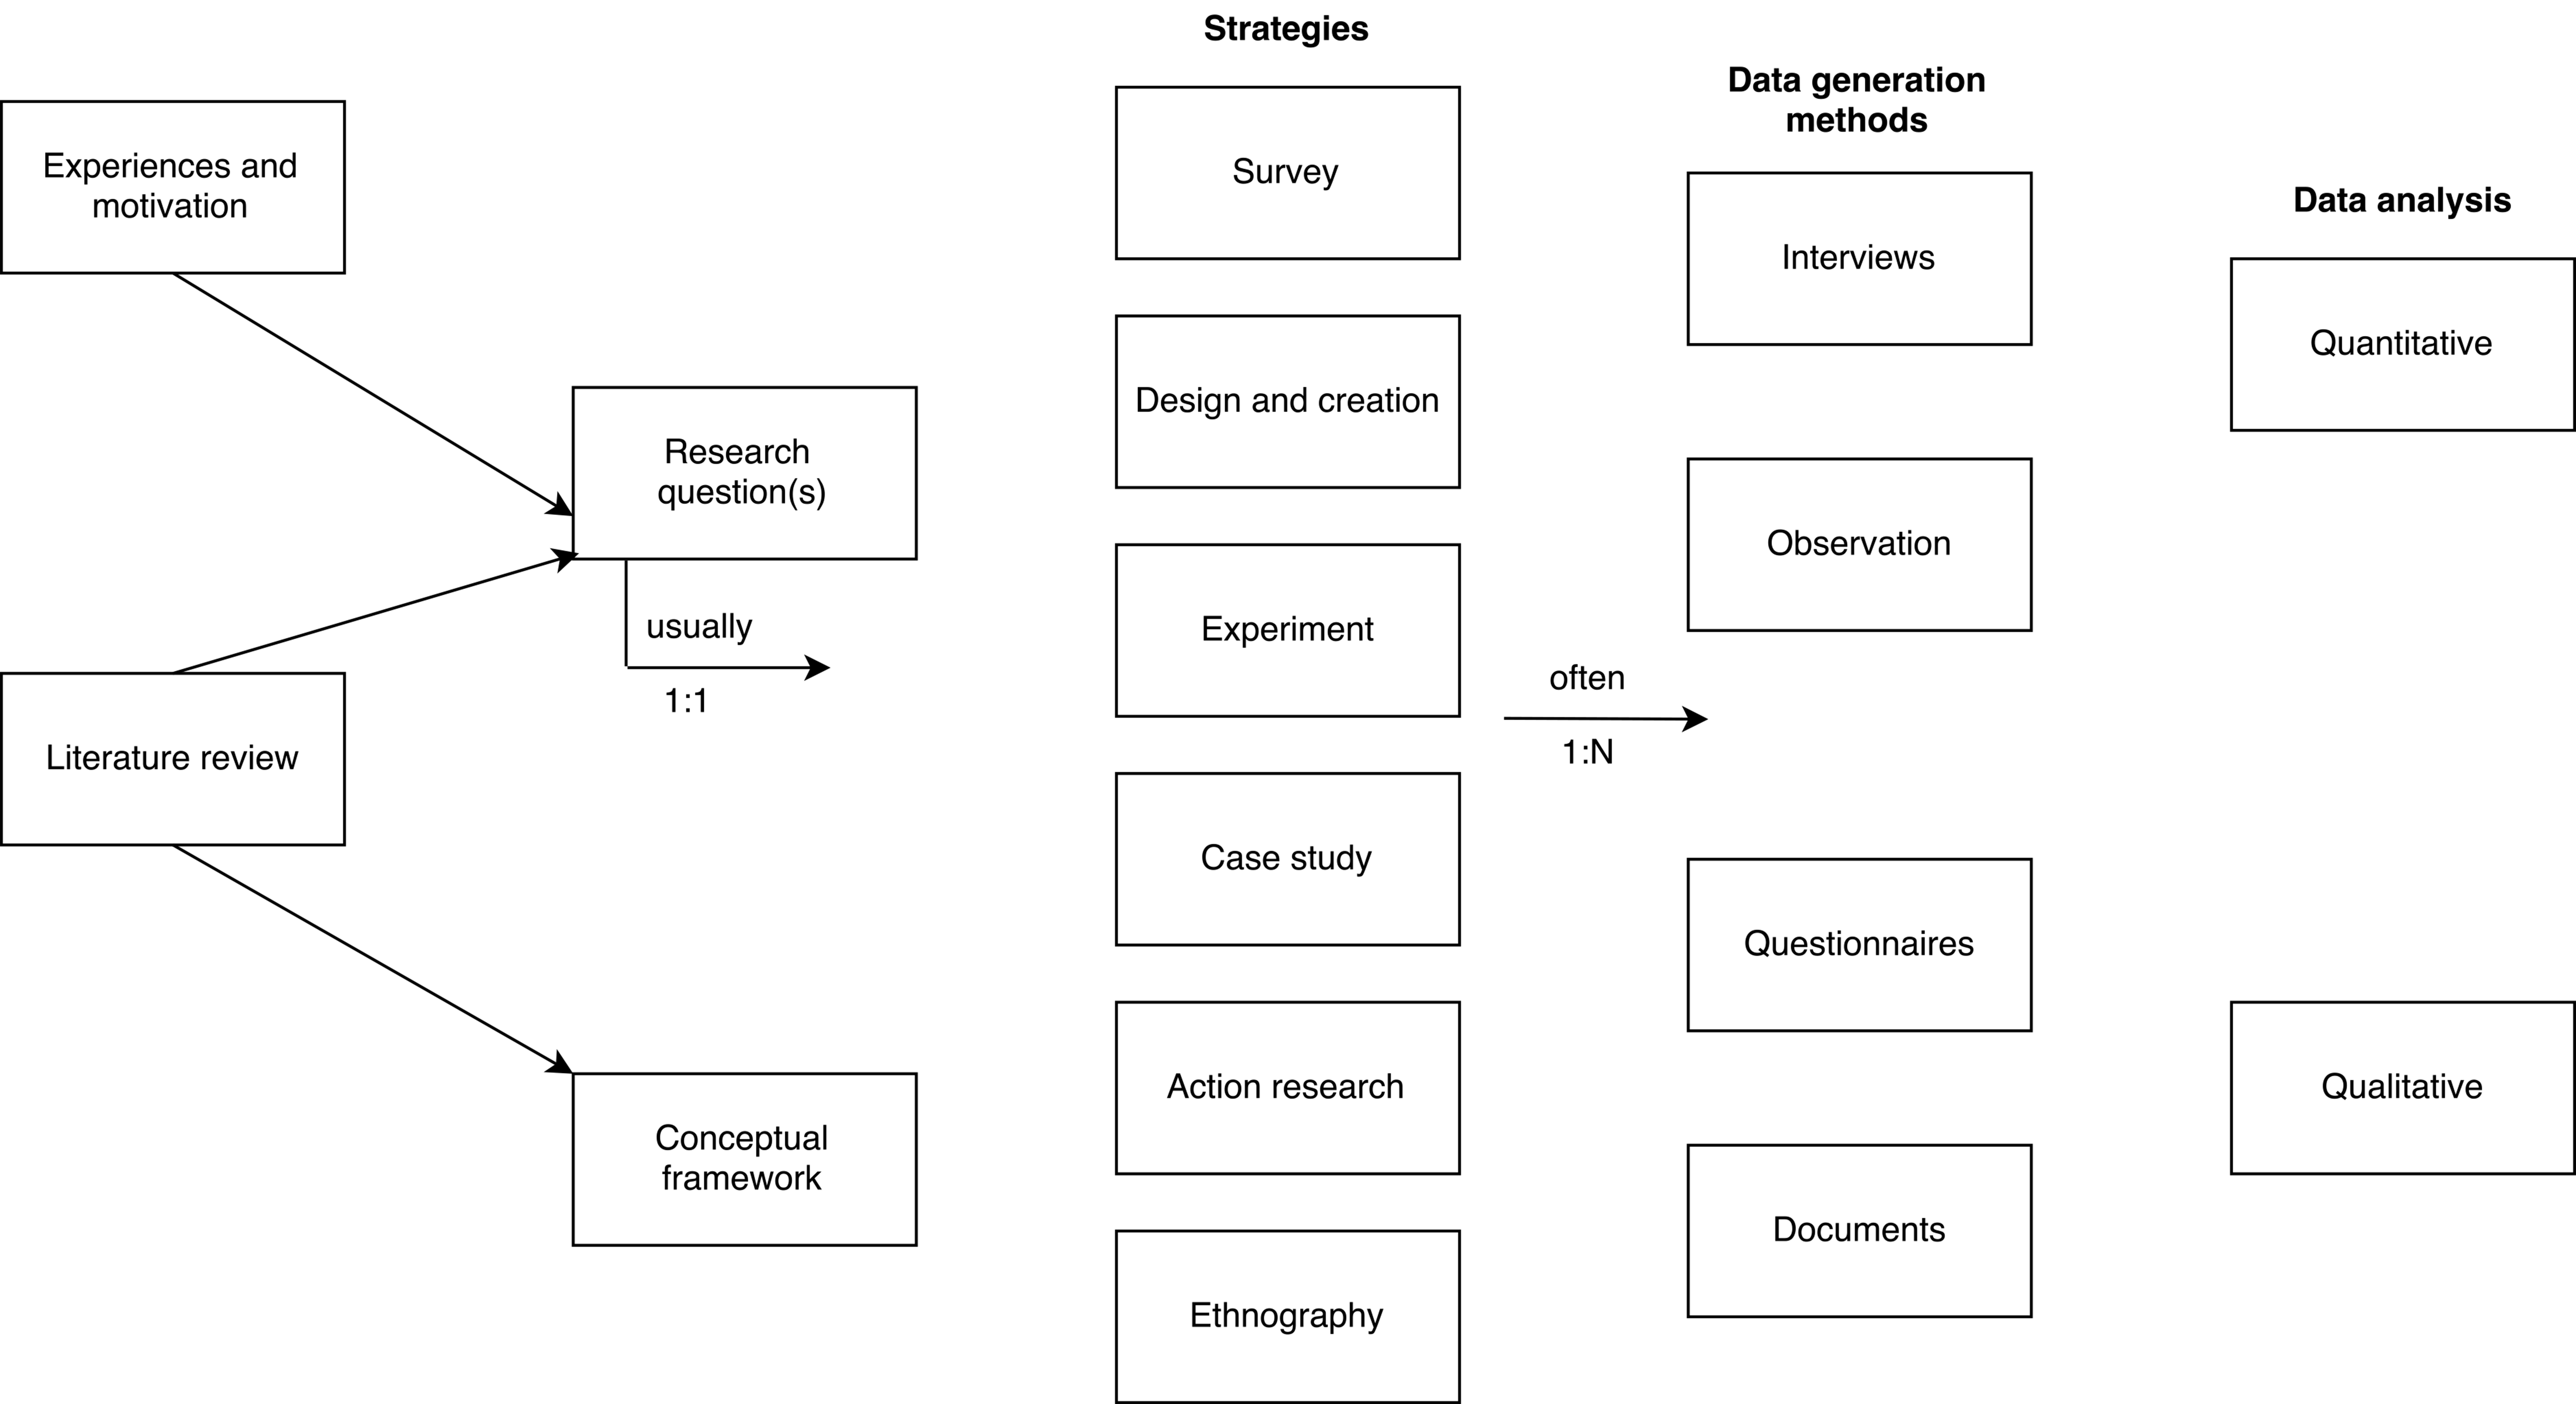
\includegraphics[width=1\textwidth]{fig/methodology/research_strategies.png}
    \caption{Model of the research process}
    \label{fig:model_research_process}
\end{figure}

Our literature review is presented in Chapter \ref{ch:related_work}. The research questions were presented in Section \ref{sec:goals_and_research_questions}, and was explained further in Section \ref{sec:research_questions_and_approach}. The conceptual framework is presented throughout this chapter. Our choice of research strategy is presented in the next section, and our choice of data generation methods, as well as our data analysis approach, is presented in Section \ref{sec:data_generation_methods_and_data_analysis}.

%%=========================================

\section{Research Strategy}
\label{sec:research_strategy}
We carefully chose our research strategy based on our research questions and overarching goal, and how they could best be answered and achieved. We decided to use the research strategy of design and creation combined with the research strategy of experiments. \cite{oates2005researching} states that it is most common to use a single research strategy, but that it is also possible to combine one or more. Our combination of research strategies allowed us to build one or more models iteratively, and to test various approaches to find optimal solutions. We followed the strategy of design and creation for the most part, but utilized experiments to investigate cause and effect relationships. The results from the experiments were later used to progress. We also used experiments to answer the research questions, which would be an important part of our research.

\subsection{Design and Creation}
\label{sec:design_and_creation}
Development of a new IT product is the primary focus of the design and creation research strategy. IT products are also called artefacts, and there are four of these \citep{march1995design, oates2005researching}:

\begin{itemize}
    \item\textbf{Constructs:} the concepts or vocabulary used in a particular IT-related domain. For example, notions of entities, objects or data flow.
    \item\textbf{Models\footnote{Note that \cite{oates2005researching} uses this term for something else than what the ``industry'' term implies. Outside this chapter, we use the term ``model'' as the term ``instantiations'' defined by \cite{oates2005researching}}:} combinations of constructs that represent a situation and are used to aid problem understanding and solution development. For example, a data flow diagram, a use case scenario or a storyboard.
    \item\textbf{Methods:} guidance on the models to be produced and process stages to be followed to solve problems using IT. For example, formal, mathematical algorithms, or commercialized and published methodologies.
    \item\textbf{Instantiations:} a working system that demonstrates that constructs, models, methods, ideas, genres or theories can be implemented in a computer-based system.
\end{itemize}

In our case, the artefact we wanted to develop as a part of our research would fall into the category of instantiations. This artefact would be a fully functional system that would be capable of achieving our research goal, as well as answering our research questions.  As this system would be an essential part of the research process, it would be important that it could be considered as research, and not just as a demonstration of technical powers. The process and the development of the system had to demonstrate academical qualities such as analysis, explanation, argument, justification, and critical evaluation \citep{oates2005researching}. 

\subsubsection{Approach}
\label{methodology-design-and-creation-approach}
The approach in design and creation revolves around a problem-solving strategy. It utilizes an iterative process over five steps \citep{vaishnavi2004design, oates2005researching}:

\begin{itemize}
    \item\textbf{Awareness:} involves recognizing a problem. This step is necessary to find what problem we are trying to solve.
    \item\textbf{Suggestion:} is the step where we create a tentative idea of how the problem might be addressed.
    \item\textbf{Development:} is where we implement an idea from the previous step.
    \item\textbf{Evaluation:} involves examining the artefact. Evaluations are done to estimate its worth and deviations from the expectations.
    \item\textbf{Conclusion:} is the final step in the cycle where results are collected and written down. Gained knowledge is identified, and any unexpected or unexplainable results could lay the ground for further research.
\end{itemize}

It is important to understand that these steps are not necessarily followed in a strict manner. Instead, they work as guidelines, and the process is more of an iterative fluid cycle where the approach may shift depending on problem or situation. \cite{oates2005researching} explains how these cycles work and what you as a researcher achieves by using this research method as follows:

\begin{quote}
    Thinking about a suggested tentative solution leads to greater awareness of the nature of the problem; development of a design idea leads to increased understating of the problem and new, alternative tentative solution; discovering that a design doesn't work according to the researcher's expectations leads to new insights and theories about the nature of the problem, and so on. 
\end{quote}

The goal is to work out a prototype that is gradually modified until a satisfactory implementation is produced. One of the biggest advantages of this approach is that it is not necessary to fully understand a problem before developing prototypes and exploring tentative solutions. This research strategy also opens up the possibilities of testing prototypes often and comparing results along the way to see if one direction or approach works better than others. 

\subsection{Experiment}
\label{sec:experiment}
Experiments are, as already mentioned, a research strategy that focuses on investigating cause and effect, and the relationship between the two. Experiments are structured around hypothesis. With a given hypothesis, an experiment is designed to prove or disprove the hypothesis. For example, a hypothesis may be:

\begin{description}
    \item[Hypothesis:]{\textit{if I go outside in the rain, I am going to get wet.}}
\end{description}

According to \cite{oates2005researching}, research strategies that are based on experiments may, among others, be characterized by:

\begin{itemize}
    \item Observation and measurement. Here the researchers make a precise and detailed observation of outcome and changes that occur when a particular factor is introduced.
    \item Proving or disproving a relationship between two or more factors.
    \item Explanation and prediction. The researchers are able to explain the casual link between two factors.
    \item Repetition, where experiments are carried out multiple times. This repetition is done under varying conditions, to be certain that the observed and measured outcomes are not caused by some other factor.
\end{itemize}

\subsection{Combining the Two Strategies}
\label{sec:combining_the_two_strategies}
As stated earlier, we did not use both of the strategies in its complete form throughout the entire process. Instead, we lent on the fluid nature of design and creation, and we used concepts from experiments to help us move forward. 

We created meaningful hypothesis related to the current tentative solution for a problem. While implementing the solution, we also made sure to construct it in such a way that we could test our hypothesis when it was finished. We evaluated the results of the development process and cross-examined them with the results from the experiments. The combined knowledge gained though this approach helped us in the next cycle of development by uncovering how to proceed.

%%=========================================

\section{Data Generation Method and Data Analysis}
\label{sec:data_generation_methods_and_data_analysis}
Data generation method is the means by which we produced the empirical data on which we evaluated our research. As stated by \cite{oates2005researching}, many researchers who chose to use the design and creation strategy pay little attention to properly use the data generation methods as presented in their research approach model. This is usually because the artefact that is developed needs to be tested in a specific way. Evaluation of a system like ours is often done by training and testing it on sets of data. Such data generation methods fall outside the overview presented in Figure \ref{fig:model_research_process}. We generated datasets and tested the system on these sets.

Data analysis based on the data from our tests was done quantitatively. Quantitative data analysis means that our data and evidence were based on numbers. The data was compared and analyzed using tables, charts, and graphs. Developing a system iteratively, as we did, this type of analysis made it easier to compare results, behavior, and progression.